\section{Algorithme d'apprentissage}


Le principe de l'apprentissage machine est le suivant: nous avons un estimateur à qui nous envoyons deux jeux de données. Une matrice X qui représente les données à évaluer et une matrice Y qui représente les résultats correspondant aux données. 
Des hypers-Paramètres lui sont également envoyé afin que le modèle puisse estimer correctement le paramètre $\theta$. 
(voir~\autoref{fig:Apprentissage_Machine})

\begin{figure}[htpb]
	\centering
	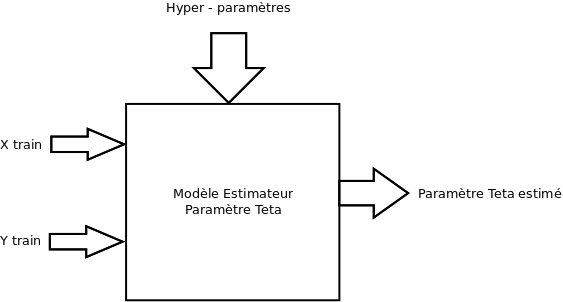
\includegraphics[scale = 0.25]{images/Diagramme1}
	\caption{Schéma d'apprentissage Machine}
	\label{fig:Apprentissage_Machine}
\end{figure}

Ici, l'estimation du paramètre $\theta$ doit être tel que l'erreur estimé sur les prédictions soit le minimum possible. 
Cette erreur est estimée selon un modèle de régression linéaire qui doit minimiser selon le paramètre $\theta$ par la méthode des moindres carrés, c'est-à-dire minimiser la formule suivante : 

\begin{equation}
erreur = \sum_{i=1}^{n} (|y_{i} - \hat{y}_{i}|^{2})
\end{equation}
avec $y_{i}$ les vrais résultats et $\hat{y}_{i}$ les résultats estimés. 

Une fois que l'erreur a été estimé et que les $\theta$ ont été calculé, il est testé sur un échantillon test, suite à cela, la machine calcul une prédiction des résultats qu'on compare aux vrais résultats (voir~\autoref{fig:Apprentissage_Machine_Prediction}). 

\begin{figure}[htpb]
	\centering
	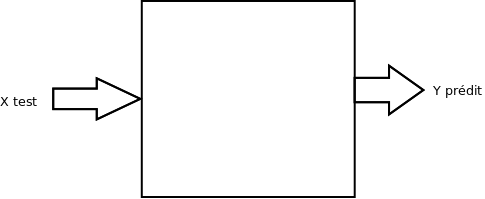
\includegraphics[scale = 0.25]{images/App_Mach_Prediction}
	\caption{Schéma d'apprentissage Machine}
	\label{fig:Apprentissage_Machine_Prediction}
\end{figure}

\todo{expliquer l'apprentissage des k voxels}
